\documentclass{standalone}
\usepackage{tikz}
\begin{document}
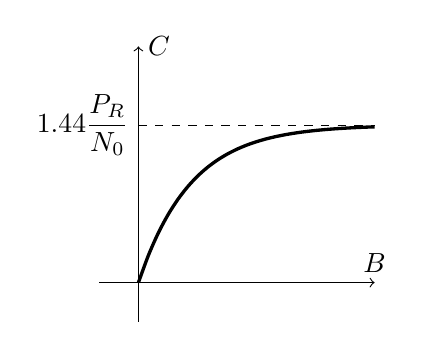
\begin{tikzpicture}[scale=2]
    \draw[->](-0.25,0)--(1.5,0)node[above]{$B$};
    \draw[->](0,-0.25)--(0,1.5)node[right]{$C$};
    \draw[very thick, smooth, domain=0:1.5]plot(\x,{1-e^(-3*\x)});
    \draw[dashed](0,1)node[left]{$1.44\displaystyle\frac{P_R}{N_0}$}--(1.5,1);
\end{tikzpicture}
\end{document}